\section{Social graphs}
\subsection{Analyzing graphs}
\begin{itemize}
\item Objects have described by attributes
\item Relations inferred from distance measures on attributes
\end{itemize}

Use of explicit relationships: graphs
\begin{itemize}
\item relationships are explicitly given
\item social network graphs
\item Graph structure can be inferred from distance measure
\end{itemize}

\subsection{Graphs and clustering}
Networks often contain structure: clusters (also called communities,
modules)

\subsection{Social network analysis}
Clusters (communities) in social networks
\begin{itemize}
\item Interests
\item Level of trust
\end{itemize}

\subsection{Community detection algorithms}
Hierarchical clustering
\begin{itemize}
\item iteratively identify groups of nodes with high similarity
\item \textbf{Agglomerative algorithms} merges nodes and community
  with high similarity
\item \textbf{Divisive algorithms} split communities by removing links
  that connect nodes with low similarity
\end{itemize}

\subsection{Louvain modularity algorithm}

Agglomerative community detection
\begin{itemize}
\item Based on \textbf{modularity} measure
\item greedy optimization of modularity
\end{itemize}

Overall
\begin{itemize}
\item first small communities are found by optimizing modularity
  locally
\item then each small community is grouped into on new community node
\item repeat till no more new communities
\end{itemize}

\subsubsection{Measuring community quality}
Communities are sets of nodes with many mutual connection, and much
less connection to outside. \textbf{Modularity} measures this(higher =
better) \\
$ \sum_{C \in communities} (\#edges within c - expected \# edges
within c )$

\subsubsection{Expected number of edges}
Graph with unweighted edges
\begin{itemize}
\item $ m $ = total number of edges
\item $ k_i $ = number of outgoing edges of node i (degree)
\end{itemize}
Observation: there is 2m ``edge ends''. Assume that all nodes receive
a fraction of $ \frac{k_i}{2m} $ edges from node i.

\subsubsection{Modularity}
Modularity measure Q
\begin{itemize}
\item $ A_{ij} $ = effective number of edges between i and
\item $ c_i, c_j $ = communities of i and j
\item $ Q = \frac{1}{2m} \sum_{i, j} (A_{ij} - \frac{k_i
    k_j}{2m})\delta(c_i, c_j) $
\item $ \delta(c_i, c_j) = 1 $ if $ c_i = c_j $ so we only consider§
  nodes from the same community
\item $ Q \in [-1, 1] $
\item $ Q > [0.3, 0.7] $ means significant community structure
\end{itemize}

\subsection{Optimizing modularity}
What we gain by moving i to the community of any neighbor? Test all
and choose best. Then merge nodes in the same community and
re-run. Modularity can be used to evaluate the best level of cutoff of
a hierarchical clustering. \\

Louvain widely used in social net analysis. Extract communities from
very large networks fast: \textbf{O(n log n)}

\subsection{Girvan Newman algorithm}
Divisive community detection
\begin{itemize}
\item Based on \textbf{betweenness measure} for edges, measuring how
  weel they separate communities
\item Decompose network by splitting along edges with highest
  separation capacity
\end{itemize}

Algorithm
\begin{itemize}
\item Repeat until no edges left
  \begin{itemize}
  \item Calculate betweenness
  \item Remove edge with highest
  \item Connected components are community
  \end{itemize}
\item  Results in hierarchical decomposition
\end{itemize}

Edge betweennesss = Number of shortest paths going through the
edge. If multiple shortest paths exist among two nodes split the flow
entirely.

\subsubsection{Computing betweenness - BFS}
\begin{itemize}
\item Perform BFS starting from A $ \forall A \in G $
\item Count the number of shortest paths from A to all other nodes
  $ \#shorttestpaths(A - X) = \sum_{P parent of X} = \#shortestpaths(A -
  P) $
\item Edge flow: working up the tree: if multiple paths count them
  fractionally to number of paths to node
\end{itemize}
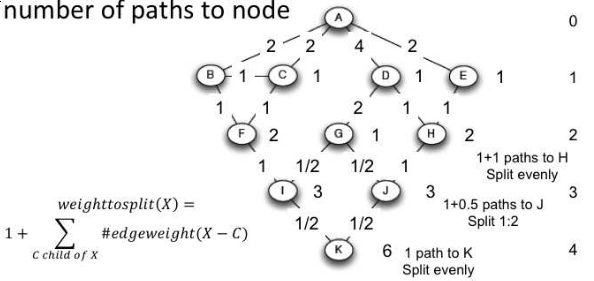
\includegraphics[width=150px,height=90px]{edgeflow}

\subsubsection{Algorithm betweenness}
\begin{itemize}
\item Build one BFS for each node
\item Determine edge flow for each edge
\item Sum up the flow values for each edge in all BFS to obtain
  betweenness (flows are computed between each pair so divide by 2)
\end{itemize}

\subsubsection{Girvan-Newman discussion}
\begin{itemize}
\item Works for smaller networks
\item Computation of betweenness for one link: $ O(n^2) $
\item Computation of betweenness for all links: $ O (L n^2) $
\item Sparse matrix: $ O(n^3) $
\end{itemize}

%%% Local Variables:
%%% mode: latex
%%% TeX-master: "master"
%%% End:
